\chapter{Higgs Phenomenology}
\label{sec:pheno}

%Dasu -
%The pheno chapter need not start from the Dirac equation and build up. It should have crisp intro to Higgs phenomenology starting from that portion of the Lagrangian. You don't need all the myriad details of SM like the quark mixing matrices, etc.

In this chapter I provide an increasingly detailed description of the standard model
of physics, specifically in reference to the Higgs boson. I provide a basic overview of some 
properties of the Higgs boson including how it is created in a hadron collider, an overview
of the possible decay paths for a Higgs boson, and a discussion of the Higgs boson
couplings with different fundamental particles. A description of the
Higgs boson requires covering the process of electroweak symmetry breaking (EWSB) which
provides the mathematical description of the process defining the Higgs boson and the
Higgs field.

\section{Standard Model Symmetries}
Many people are attracted to physics because of the beauty they see in the patterns of nature.
PW Anderson, a physics Nobel laureate, stated, ``it is only slightly overstating the case 
to say that physics is the study of symmetry''~\cite{pw_anderson:1972}.
One way of expressing many types of patterns mathematically is with symmetries, properties which 
remain invariant under certain transformations. The SM is defined by a group of symmetries
representing certain conserved properties. Specifically, the SM is represented by  the
symmetries of the unitary product group SU(3)$_{\text{C}} \,\times \,$ SU(2)$_{\text{L}} \, 
\times\,$ U(1)$_{\text{Y}}$~\cite{SLANSKY19811}.
These three terms all reflect symmetries and conserved quantities discussed below.

Electric charge ($Q$), the third component of weak isospin ($T_{3}$), and hypercharge ($Y$) act together to define a conserved 
quantity in the SM, $Q = T_{3} + \frac{Y}{2}$. This is represented by the
hypercharge U(1)$_{\text{Y}}$ symmetry group.

The two SU($n$) groups are special unitary groups which represent rotations.
In the SM, the SU(2) group provides a description of particle spin.
The ``L'' subscript for the SU(2)$_{\text{L}}$ group indicates that that it
only describes left handed fermions.
The SU(3)$_{\text{C}}$ group describes the local symmetry of color charge and
color charge conservation.


\section{Electroweak Symmetry Breaking}
Glashow, Weinberg, and Salam demonstrated a unified description of the electromagnetic force 
and weak force which merge at energies of order 100\GeV into the electroweak force,
described by the electroweak Lagrangian~\cite{Glashow:1961tr,SM1,SM3}.
The electroweak Lagrangian defines a gauge field theory which is 
invariant under the SU(2)$_{\text{L}} \, \times \, $U(1)$_{\text{Y}}$ symmetry group. 
Prior to the introduction of Electroweak Symmetry Breaking (EWSB),
the electroweak Lagrangian describes massless $\PW$ and $\PZ$ bosons.
However, as previously mentioned, the $\PW$ and $\PZ$ bosons discovered in 1983
are two of the most massive particles~\cite{AUBERT1983275,1983398}. 
The EWSB mechanism rescues what would be a colossal disagreement between theoretical prediction
and experimental results. The introduction of EWSB to the theory preserves the structure of
the electroweak interactions and succeeds in endowing the $\PW$ and $\PZ$ bosons
with mass.

Electroweak symmetry breaking is an application of spontaneous symmetry breaking to
the electroweak Lagrangian. It is achieved via the Brout--Englert--Higgs
mechanism~\cite{Englert:1964et,Higgs:1964ia,Higgs:1964pj,Guralnik:1964eu,Higgs:1966ev,Kibble:1967sv},
leading, in its minimal version, to the prediction of the existence of one physical neutral scalar particle,
commonly known as the Higgs boson. The EWSB mechanism, defined by Brout, Englert, and Higgs,
proposes a self-interacting complex doublet scalar field,
\begin{equation}
\phi = \begin{pmatrix} \phi_{\alpha} \\ \phi_{\beta} \end{pmatrix} = 
    \sqrt{\frac{1}{2}} \begin{pmatrix}\phi_{1} + i\phi_{1} \\ \phi_{3} + i\phi_{4} \end{pmatrix},
\label{eqn:phi_doublet}
\end{equation}

that is applied to the electroweak Lagrangian, 
\begin{equation}
\mathcal{L} = \big(D_{\mu}\phi\big)^{\dagger} \big(D^{\mu}\phi\big) - V\big(\phi\big),
\end{equation}

where $D^{\mu}$ is the covariant derivative and the potential, $V\big(\phi\big)$, 
is expressly defined with two terms, 
\begin{equation}
V\big(\phi\big) = \mu^{2}\phi^{\dagger}\phi + \lambda\big(\phi^{\dagger}\phi\big)^{2}
\label{eqn:v_pot}
\end{equation}

The Lagrangian describes a system of four scalar particles, the $\phi_{i}$,
of equation~\ref{eqn:phi_doublet} each with mass $\mu$. 
To achieve EWSB, the constants in the potential $V\big(\phi\big)$ are defined such that $\mu^{2} < 0$
and $\lambda > 0$. The choice $\mu^{2} < 0$ and $\lambda > 0$ lead to a potential $V\left(\phi\right)$
as shown in Figure~\ref{fig:higgs_potential}. Expanding around a chosen minima of the potential
$V\big(\phi\big)$, $v$, and taking $\phi_{1} = \phi_{2} = \phi_{4} = 0$ and
$\phi_{3}^{2} = -\frac{\mu^{2}}{\lambda} \equiv v^{2}$, $\phi$ becomes
\begin{equation}
\phi = \sqrt{\frac{1}{2}} \begin{pmatrix} 0 \\ v \end{pmatrix},
\label{eqn:phi_doublet_exp}
\end{equation}

where the scalar doublet, $\phi$ acquires a non-zero vacuum expectation value (VEV), $v \approx 246\GeV$.
In this process a neutral and two charged massless Goldstone bosons~\cite{PhysRev.127.965} are generated. These Goldstone
bosons mix with the fields corresponding to the broken SU(2)$_{\text{L}} \,\times\,$ U(1)$_{\text{Y}}$
symmetries giving masses to the $\PW$ and $\PZ$ bosons. The single remaining component of the
original complex doublet $\phi$ becomes a new fundamental scalar particle 
known as the Higgs boson with a mass
\begin{equation}
\mH^{2} = 2\lambda v^2,
\end{equation}
but the value of this is not predicted.

%Applying EWSB to the SM takes the symmetries expressed as 
%SU(3)$_{\text{C}} \,\times \,$ SU(2)$_{\text{L}} \,\times \,$ U(1)$_{\text{Y}}$ and turns them into
%SU(3)$_{\text{C}} \, \times \,$ U(1)$_{\text{em}}$.

\begin{figure*}[htbp]
\centering
     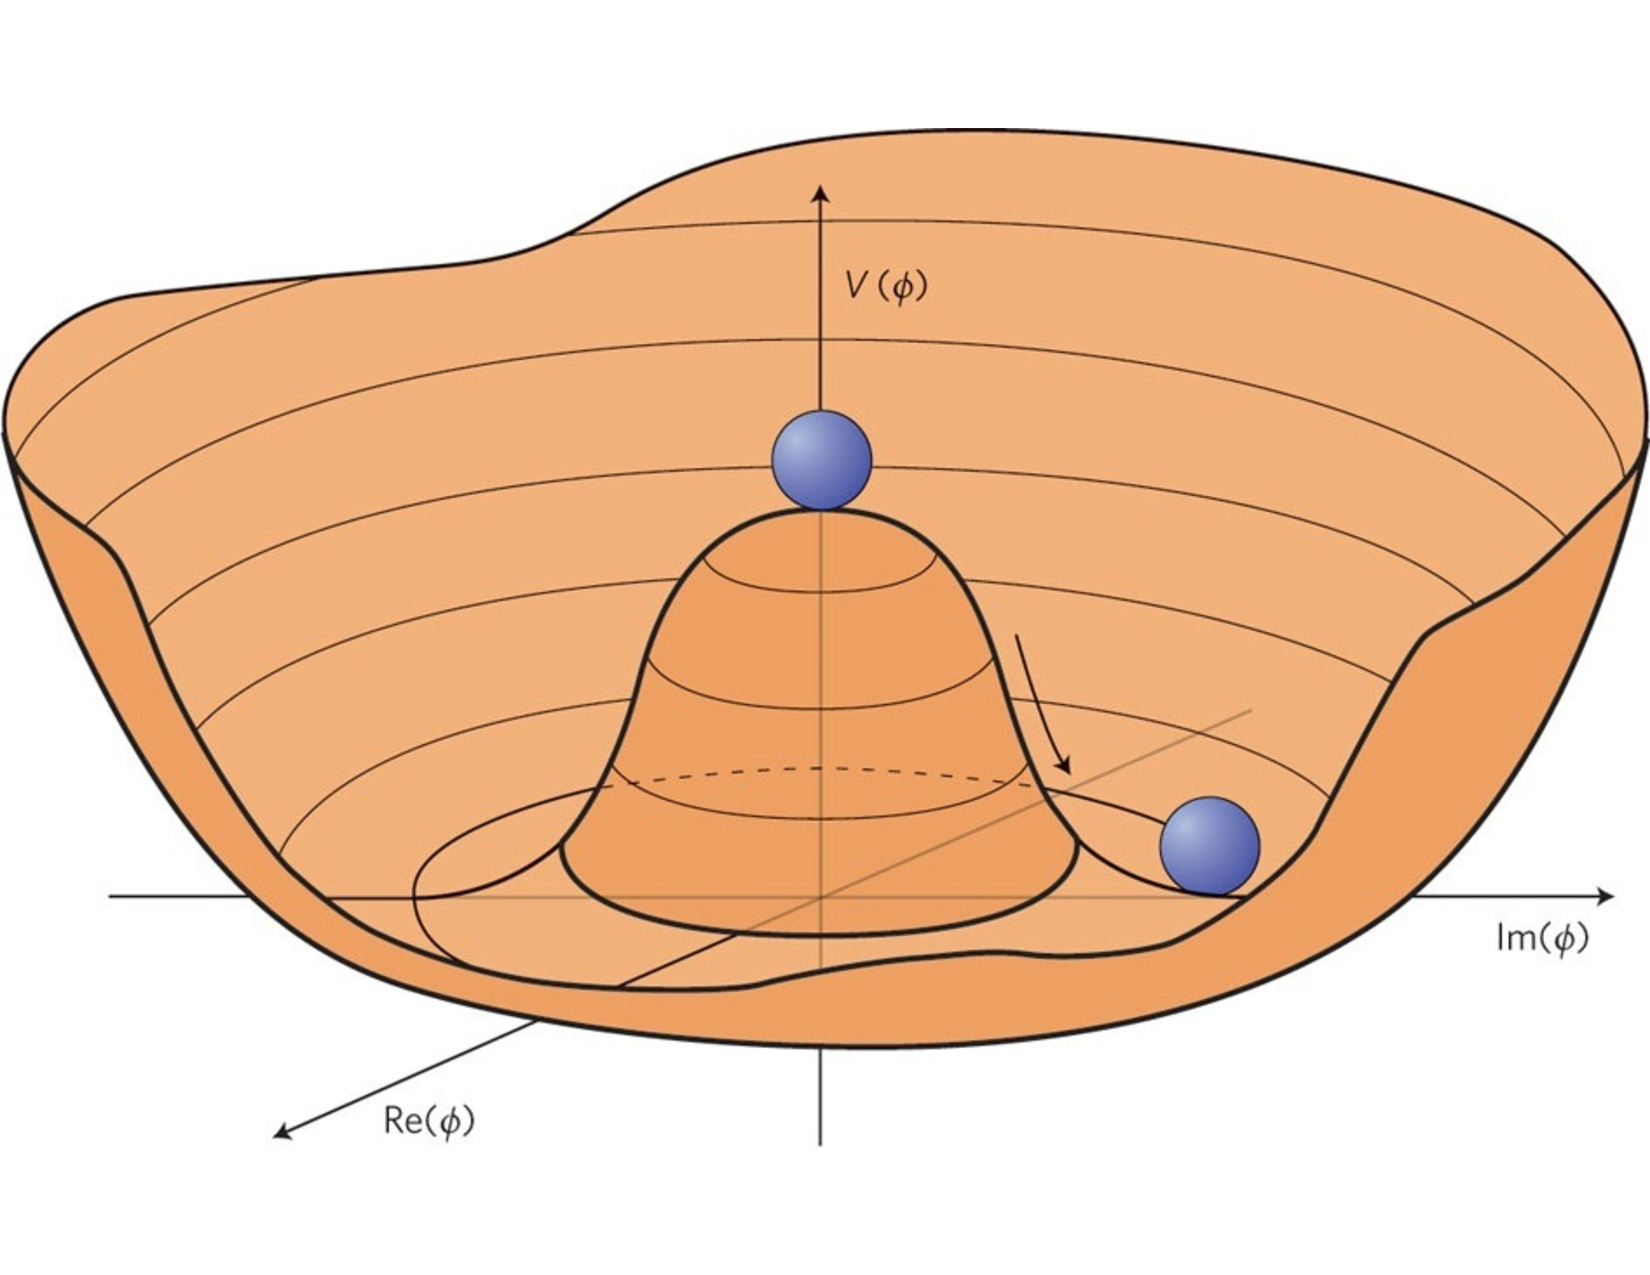
\includegraphics[width=0.55\textwidth]{phenomenology_of_processes/plots/higgs_potential.pdf}
     \caption{
The potential $V\left(\phi\right)$ from Equation~\ref{eqn:v_pot} showing a non-stable state
at the origin and a stable state in the circular trough.
     }
     \label{fig:higgs_potential}
\end{figure*}



\section{Higgs Yukawa Couplings}
In addition to providing a mechanism for the $\PW$ and $\PZ$ bosons to gain mass in the SM, the EWSB mechanism also
provides a mechanism for the fermions to acquire mass through their interactions with the Higgs boson
via Yukawa couplings. A Yukawa coupling is an interaction between a scalar field and a Dirac field
similar to,
\begin{equation}
V \approx h_{f}\bar{\psi_{f}}\phi\psi_{f},
\end{equation}

where the Dirac fields, $\psi$, describe fermions and the scalar field, $\phi$, is taken to be that of the Higgs boson. 
The introduction of a Yukawa interaction linking together the fermions and the Higgs boson,
results in massive fermions where their mass can be written as,
\begin{equation}
m_{f} = \frac{h_{f} v}{\sqrt{2}},
\label{eqn:yukawa_c}
\end{equation}

which covers the masses for the nine charged fermions: the three charged leptons and six quarks.
Neither the EWSB mechanism nor the Yukawa interaction provide insight into the larger variety of fermion
masses. Instead, the fermion masses are taken as free parameters of the SM and the values
$h_{f}$ represent the Yukawa coupling parameter for each of the fermions.

The mass of nine charged fermions are known experimentally, most to very high precision.
The $\Pgt$ lepton is known to be $1776.82\pm0.16\MeV$~\cite{PDG}.
Knowing this, the $\Pgt$ lepton to Higgs boson Yukawa coupling can be calculated from 
Equation~\ref{eqn:yukawa_c} and compared against experimental results. 
Exploring the multiple Higgs boson to fermions decay processes is the most promising way to directly probe
the Higgs boson Yukawa couplings. The Higgs boson decay process are discussed below in 
Section~\ref{sec:higgs_decays} where this discussion continues.

%with equation~\ref{eqn:yukawa_c},
%\begin{equation}
%h_{\Pgt} = \frac{\sqrt{2} \, m_{\Pgt}}{v} = \sqrt{2}\frac{1.78\GeV}{246\GeV} = 0.0102
%\label{eqn:yukawa_tau}
%\end{equation}



\section{Higgs Production}
\label{sec:higgs_production}
The Higgs boson is produced through interactions with the particles it couples to in the SM
Lagrangian. Understanding the different production mechanisms for the Higgs boson
allows experimentalists to search for unique signatures in collisions to better
help separate Higgs bosons from the myriad other interactions occurring in collisions at the LHC.
At a hadron collider like the LHC, the relevant Higgs boson production
mechanisms begin from initial states of quarks and gluons. The Higgs boson
only couples to massive particles, eliminating direct gluon to Higgs boson processes
as is seen in Figure~\ref{fig:sm_forces}.
However, the Higgs boson production process at the LHC which occurs most often
begins with two gluons in the initial state and is called gluon fusion discussed below.

Feynman diagrams of the leading Higgs boson production processes for
proton-proton based colliders are shown in Figure~\ref{fig:higgs_feyn}. 
The cross sections for the leading Higgs boson production processes for a 
center-of-mass energy of 13\TeV
are shown in Figure~\ref{fig:higgs_production}. The values for the leading
processes are approximately: gluon fusion ($ggH$) $\approx 49\pb$, 
vector boson fusion (VBF) $\approx 3.8\pb$, $\PW$ boson associated production ($\PW\PH$) $\approx 1.4\pb$,
and $\PZ$ boson associated production ($\PZ\PH$) $\approx 0.88\pb$~\cite{deFlorian:2016spz}. 
The top-quark associated process ($\ttbar\PH$),
which is found to be relatively insignificant in the following analyses, has a cross
section approximately half the size of the next smallest one, $\PZ\PH$, where
$\ttbar\PH \approx 0.51\pb$ and accounts for less than 1\% of the total Higgs boson
cross section.


\begin{figure*}[htbp]
\centering
     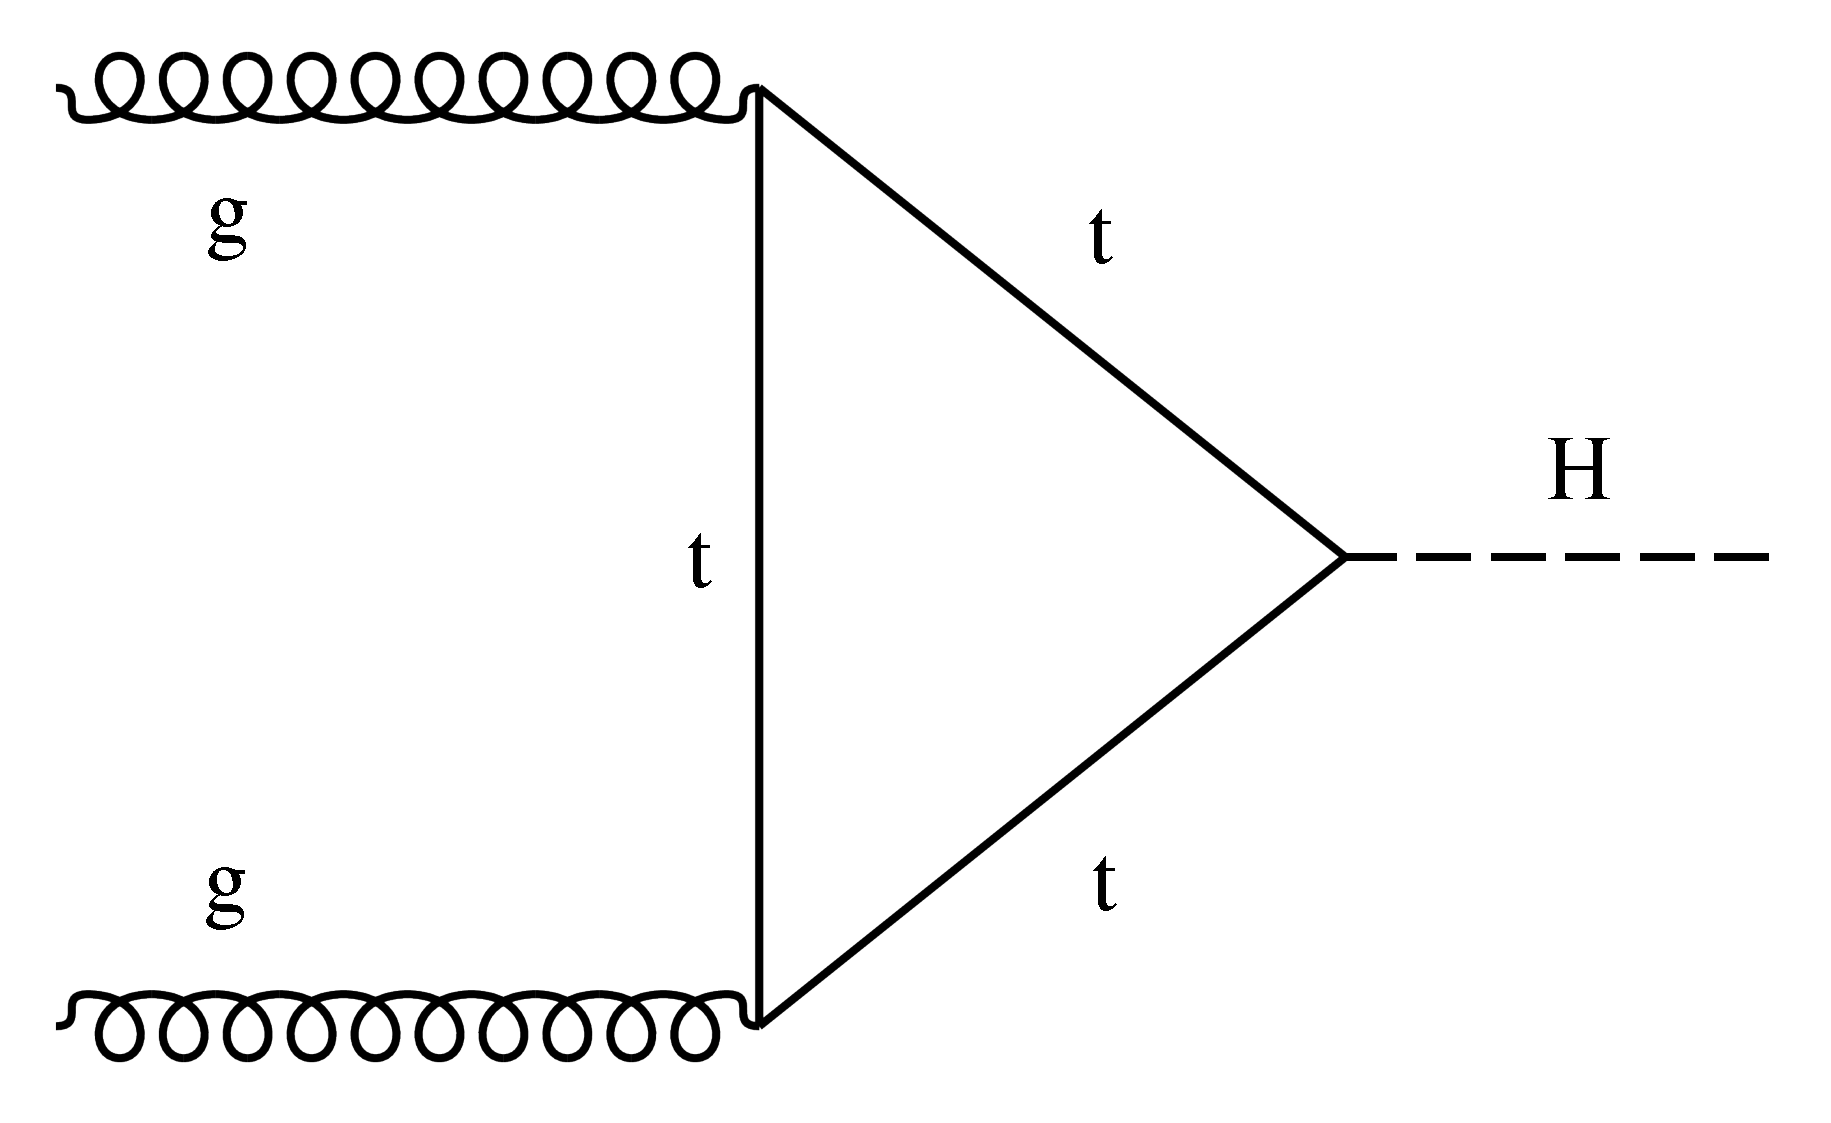
\includegraphics[width=0.35\textwidth]{phenomenology_of_processes/plots/feyn_ggH.pdf}
     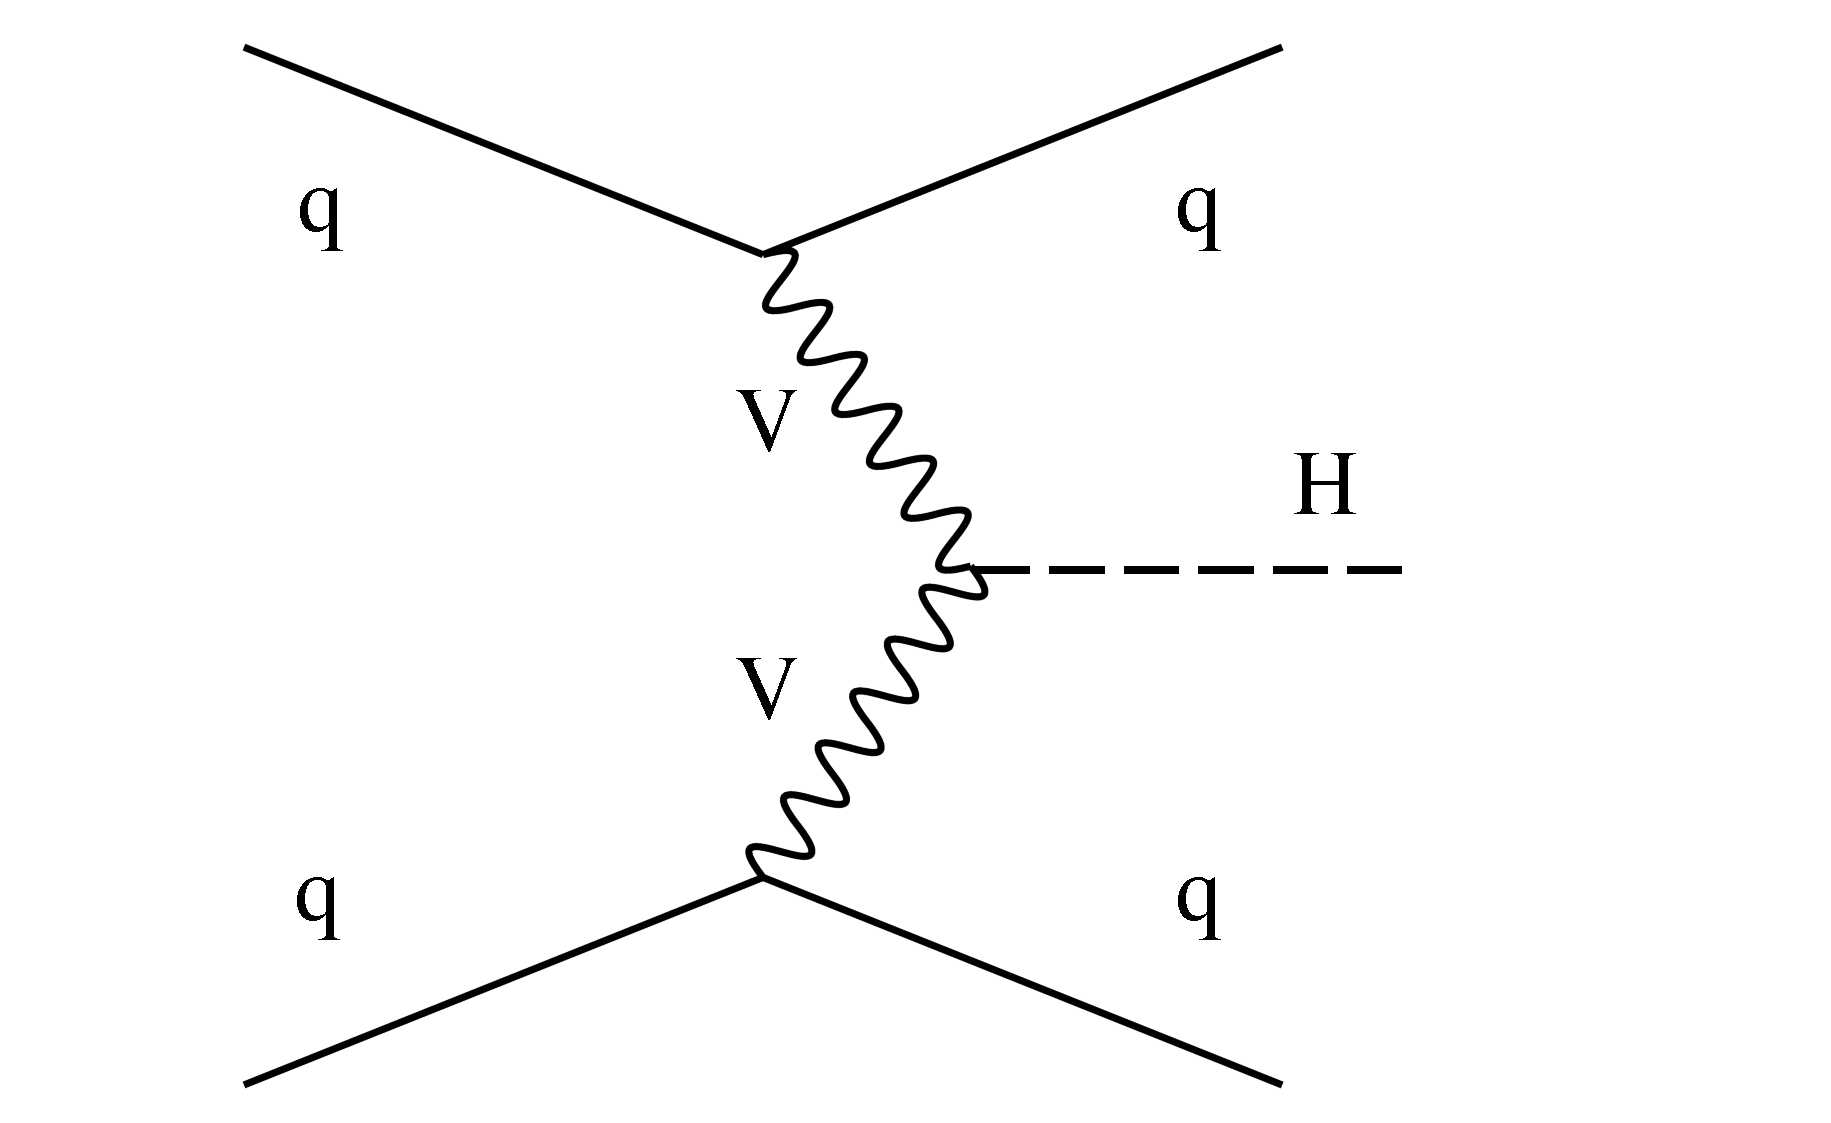
\includegraphics[width=0.35\textwidth]{phenomenology_of_processes/plots/feyn_qqH.pdf}
     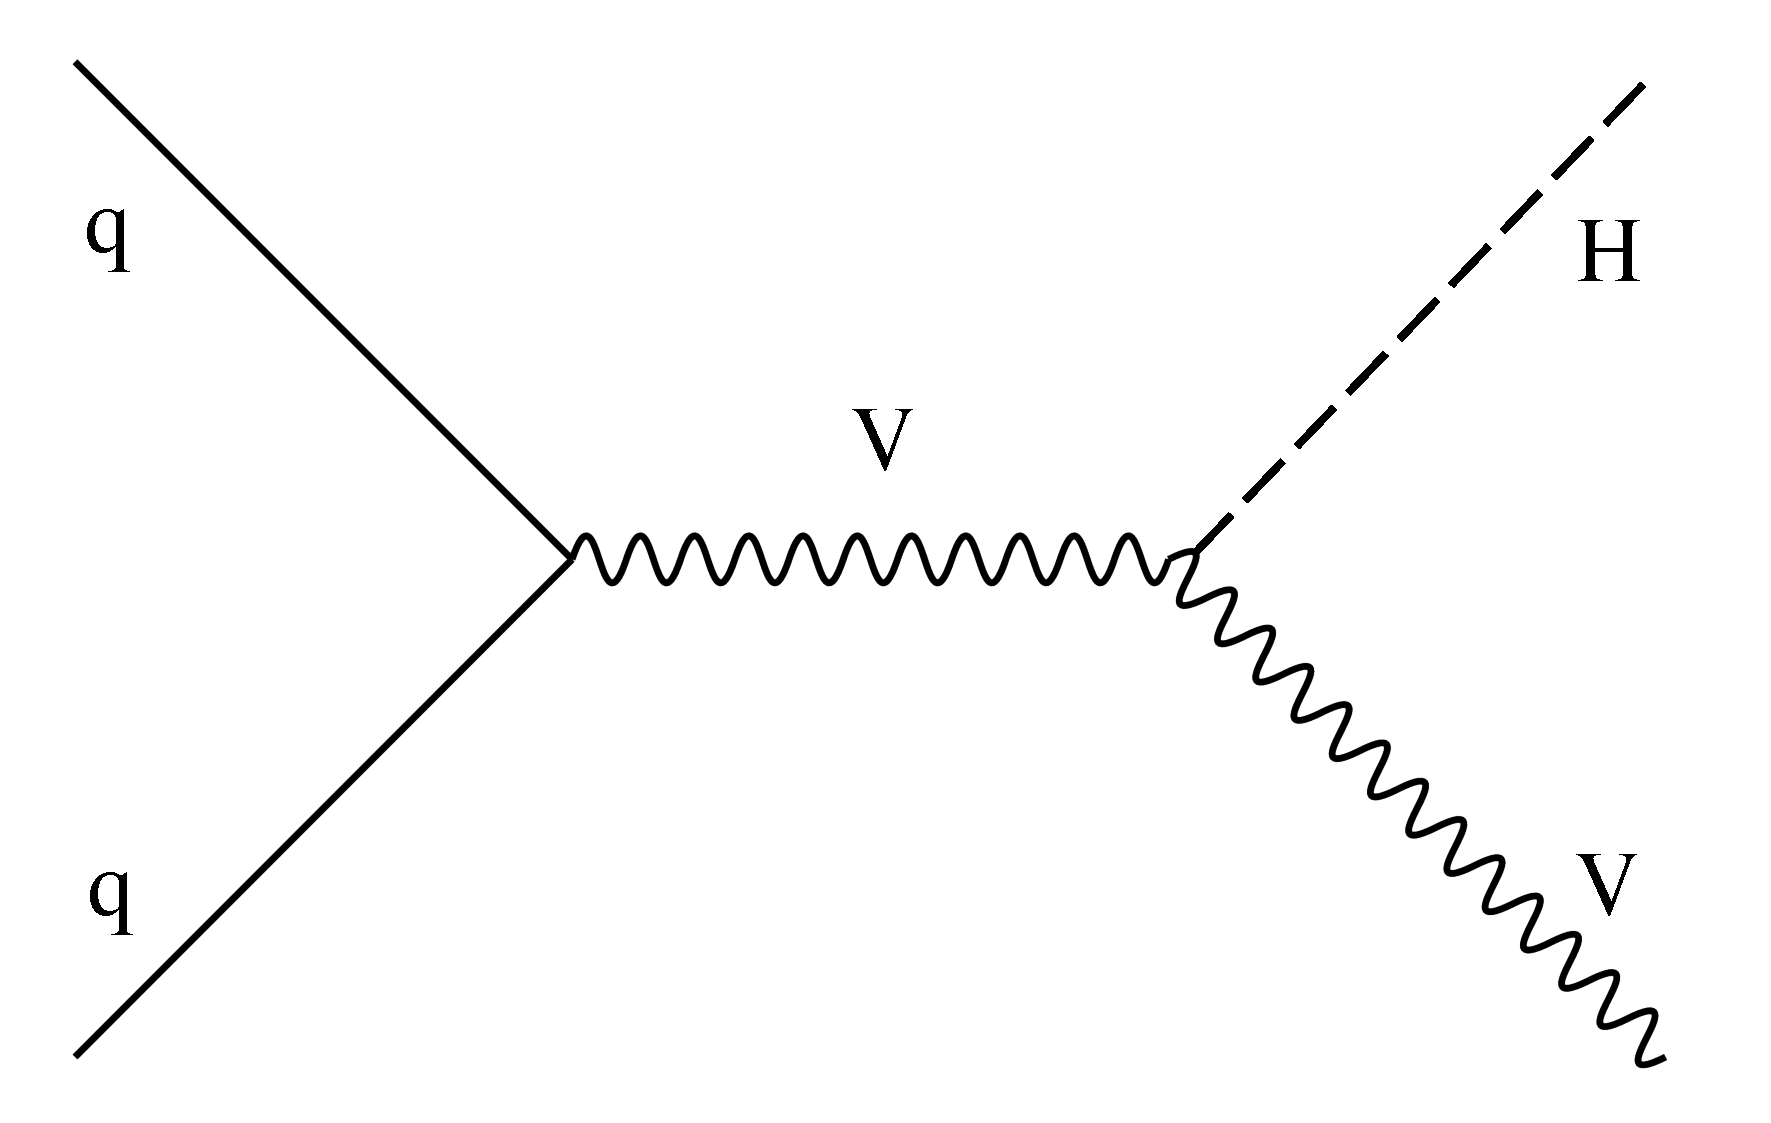
\includegraphics[width=0.35\textwidth]{phenomenology_of_processes/plots/feyn_VH.pdf}
     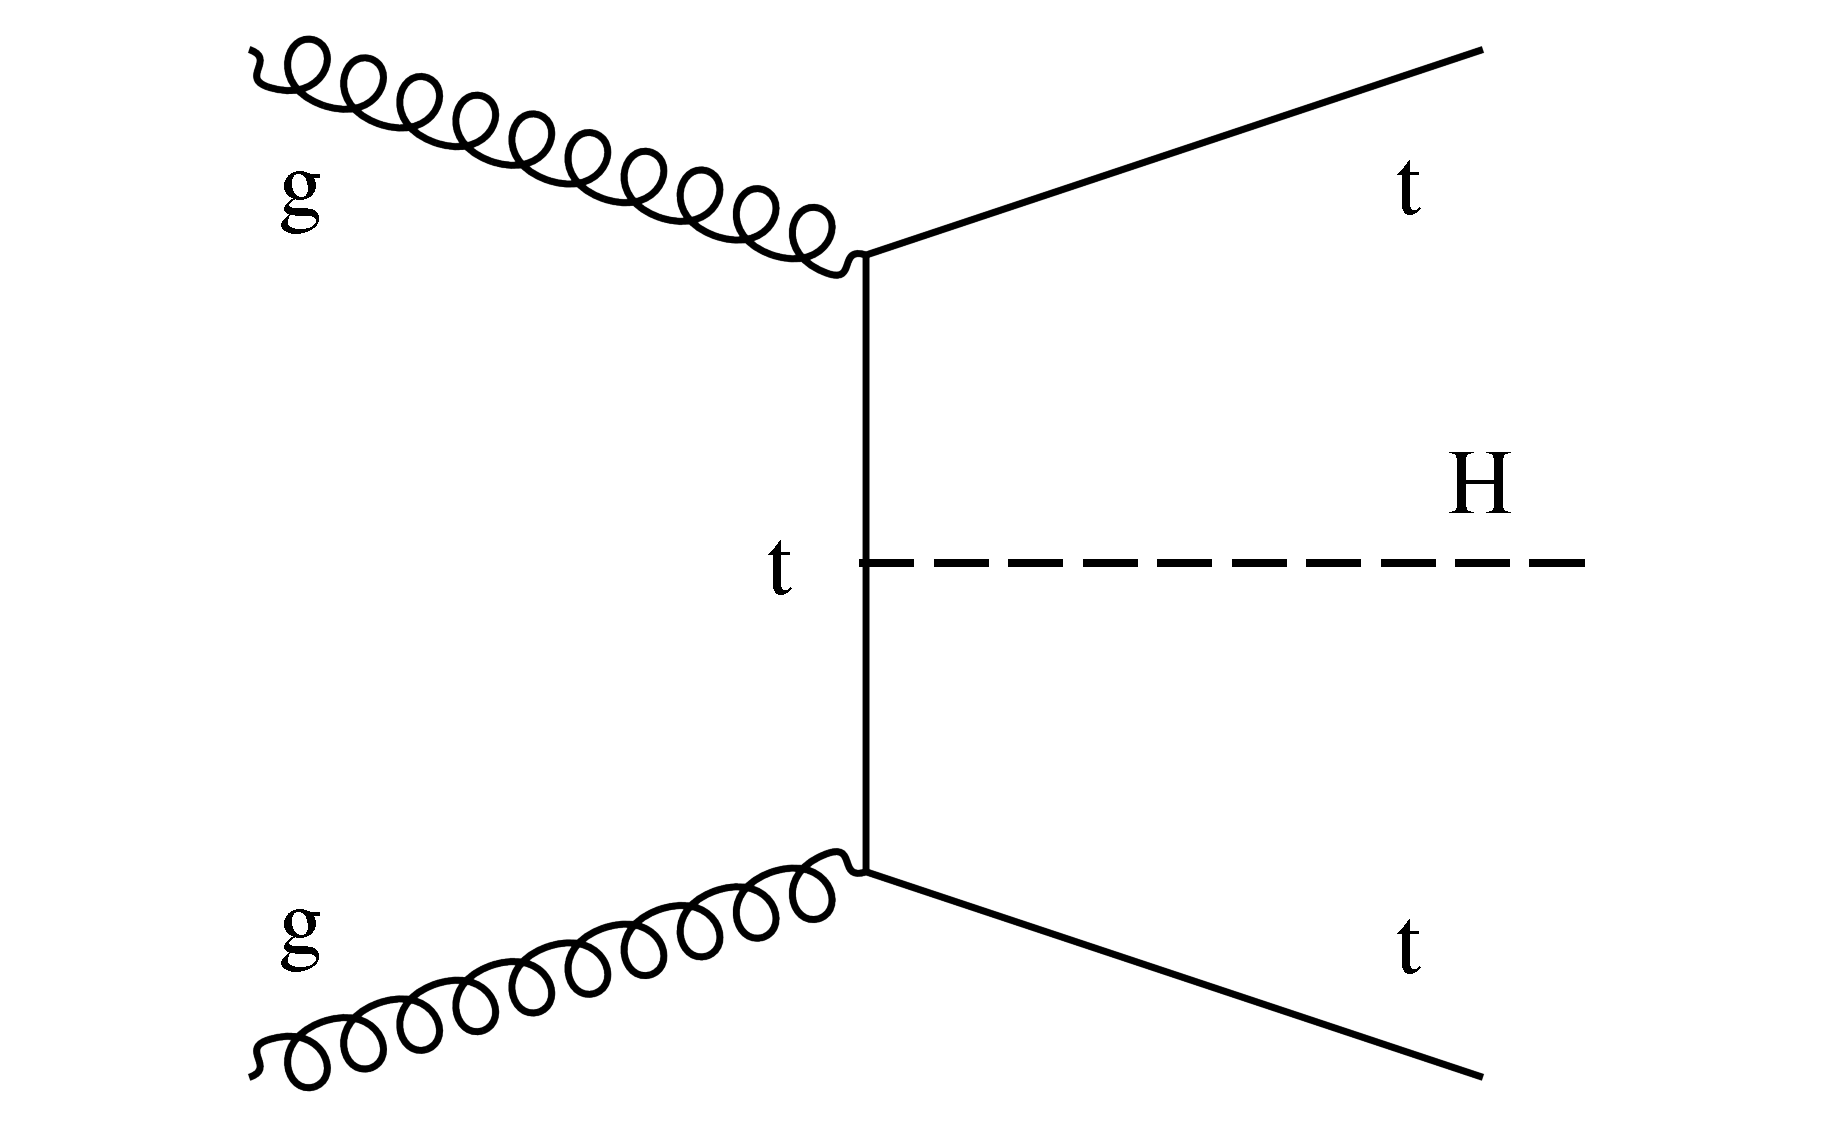
\includegraphics[width=0.35\textwidth]{phenomenology_of_processes/plots/feyn_ttH.pdf}
     \caption{
Feynman diagrams representing the leading Higgs boson production processes.
Progressing in order of largest to smallest in production cross sections:
(top left) $ggH$, (top right) VBF, (bottom left)
$\PW\PH$ and $\PZ\PH$ processes,
and (bottom right) $\ttbar\PH$.
     }
     \label{fig:higgs_feyn}
\end{figure*}


\begin{figure*}[htbp]
\centering
     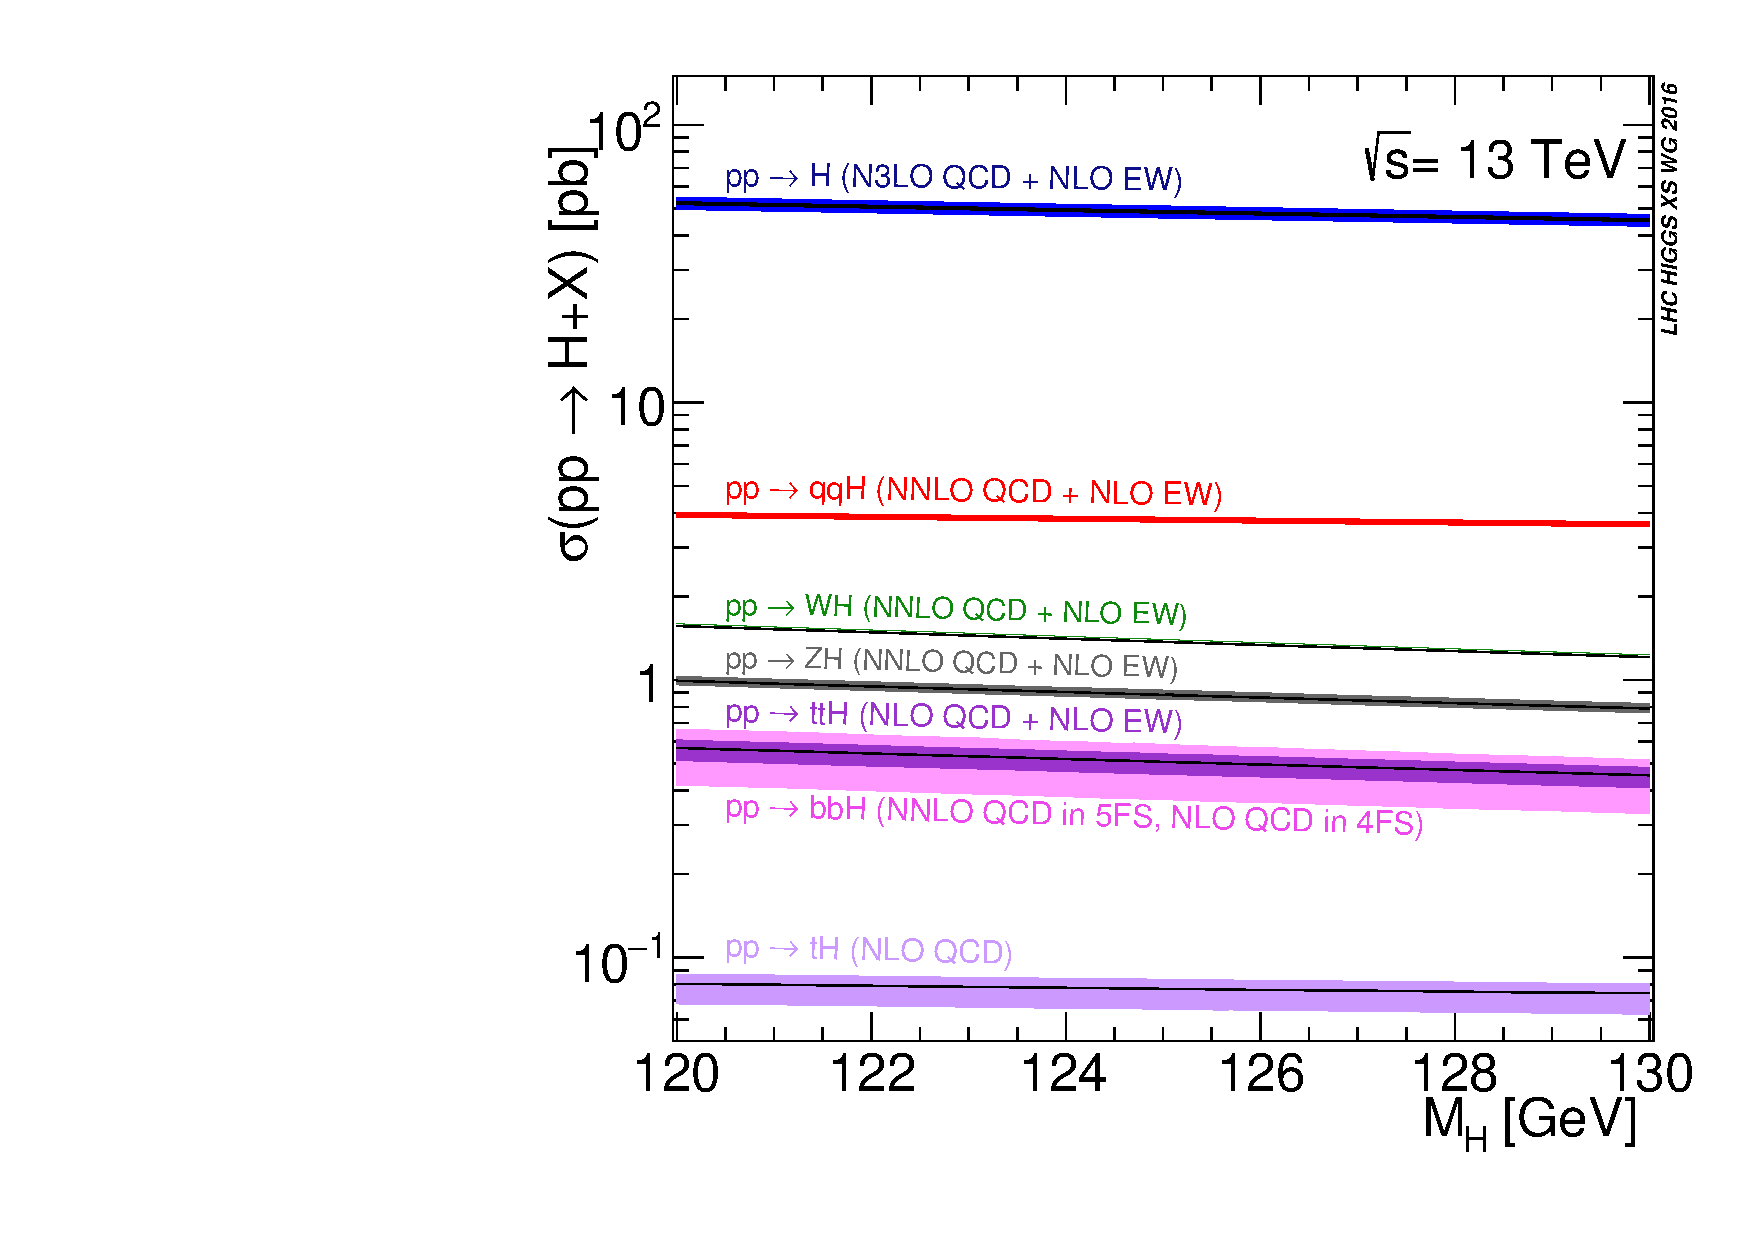
\includegraphics[width=0.65\textwidth]{phenomenology_of_processes/plots/plot_13tev_H_sqrt.pdf}
     \caption{
The calculated Higgs boson production cross sections and their uncertainties
as a function of the Higgs boson mass, are shown. The $ggH$ process
is denoted as pp $\to$ H in the figure.
The CMS and ATLAS experiments have determined $\mH = 125.09\GeV$~\cite{Aad:2015zhl}.
     }
     \label{fig:higgs_production}
\end{figure*}


\subsection{Gluon Fusion}
The Higgs boson does not couple directly to gluons. Thus, the $ggH$ process is mediated by 
a virtual top quark loop, Figure~\ref{fig:higgs_feyn}. There are contributions from the other lighter quarks; however,
their contributions in the loop are suppressed proportional to $m^{2}_{q}$.
When calculating the cross section for $ggH$, because of the relatively large mass of the top-quark, to a very good approximation, 
the leading top-quark contribution can be evaluated in the limit 
$m_{t} \to \infty$~\cite{ELLIS1976292,Shifman:1979eb}.

Despite the $ggH$ process having the largest cross section, it is the hardest process to 
isolate from background events. A portion of $ggH$ produced Higgs bosons are produced
in conjunction with one or multiple ``jets'' (``jets'' are defined in Section~\ref{sec:obj_reco_jets}).
In these cases, conservation of momentum in the transverse plane will result in the jets
and the Higgs boson recoiling off each other with their transverse momenta being
equal in magnitude and in opposite directions. This reoil can lead to a boosted topology
where the Higgs boson has a large transverse momentum
which is a unique event signature. In this thesis the boosted event topology
is used as a handle in the ``Boosted'' event selection category discussed in
Section~\ref{sec:htt_categorization}. However, the majority of $ggH$ events are produced without
additional jets. 
These events are categorized into the ``0-Jet'' category which is less sensitive because of the
lack of a clear handle to separate $ggH$ events with zero jets from the background. 


\subsection{Vector Boson Fusion}
The second largest Higgs boson production process is VBF. This process originates by
the scattering of two quarks or anti-quarks. The scattering is mediated by the t-
or u-channel exchange of a $\PW$ or $\PZ$ boson. The Higgs boson is radiated off
of the $\PW$ or $\PZ$ boson~\cite{PhysRevD.70.113009}, Figure~\ref{fig:higgs_feyn}. 
The quarks or anti-quarks which are scattered
lead to the generation of high-energy jets.
This is a highly unique event signature and is used in nearly all Higgs analyses
to identify Higgs bosons produced via VBF. In this thesis, events with two high-energy
jets consistent with VBF topology are categorized into a ``VBF'' category for analysis.


\subsection{Associated Production}
The Higgs boson associated production mechanism makes up the third and fourth largest
Higgs boson cross sections for $\PW\PH$ and $\PZ\PH$ respectively. Both processes are 
depicted in the lower left Feynman diagram in Figure~\ref{fig:higgs_feyn} where
the $V$ represents vector bosons covering both $\PW$ and $\PZ$. Associated
production is often called Higgs-strahlung in reference to bremsstrahlung which is the
process where a decelerating charged particle emits radiation, often an electron
emitting a photon. In the case of Higgs-strahlung, the vector boson created 
from two initial state quarks or anti-quarks emits a Higgs boson. The associated
production event topology is quite unique with the presence of a $\PW$ or $\PZ$
boson plus a Higgs boson. In this thesis there is an analysis targeted at each
of these process, $\PW\PH$ and $\PZ\PH$. We focuse on events where the vector
bosons decay leptonically: $\PW^{\pm} \to \ell^{\pm} + \bar{\nu}$ and $\PZ \to \ell^{+}\ell^{-}$.



\section{Higgs Boson Decays}
\label{sec:higgs_decays}
After a Higgs boson is produced, it will decay extremely rapidly with a predicted lifetime
of $1.6 \times 10^{-22}\text{s}$~\cite{Dittmaier:2012vm}. When created
inside of the CMS detector, a Higgs boson will always decay
within the LHC beampipe. In all Higgs boson analyses, experimentalists search for the
signatures of the decay products in energy deposits in their detectors, not the Higgs
boson itself. There are multiple possible decay
paths each with its own branching ratio; the largest branching ratio
processes are shown in Figure~\ref{fig:higgs_decay}. The $\htt$ process has a branching
ratio of approximately 6.3\% with a relative theoretical uncertainty of 
$\pm5.7\%$~\cite{deFlorian:2016spz} for $\mH = 125.09\GeV$. This places $\htt$ below $\PH\to\bbbar$, 
$\PH\to\PW\PW$, and $\PH\to\Pg\Pg$ in branching fraction.

\begin{figure*}[htbp]
\centering
     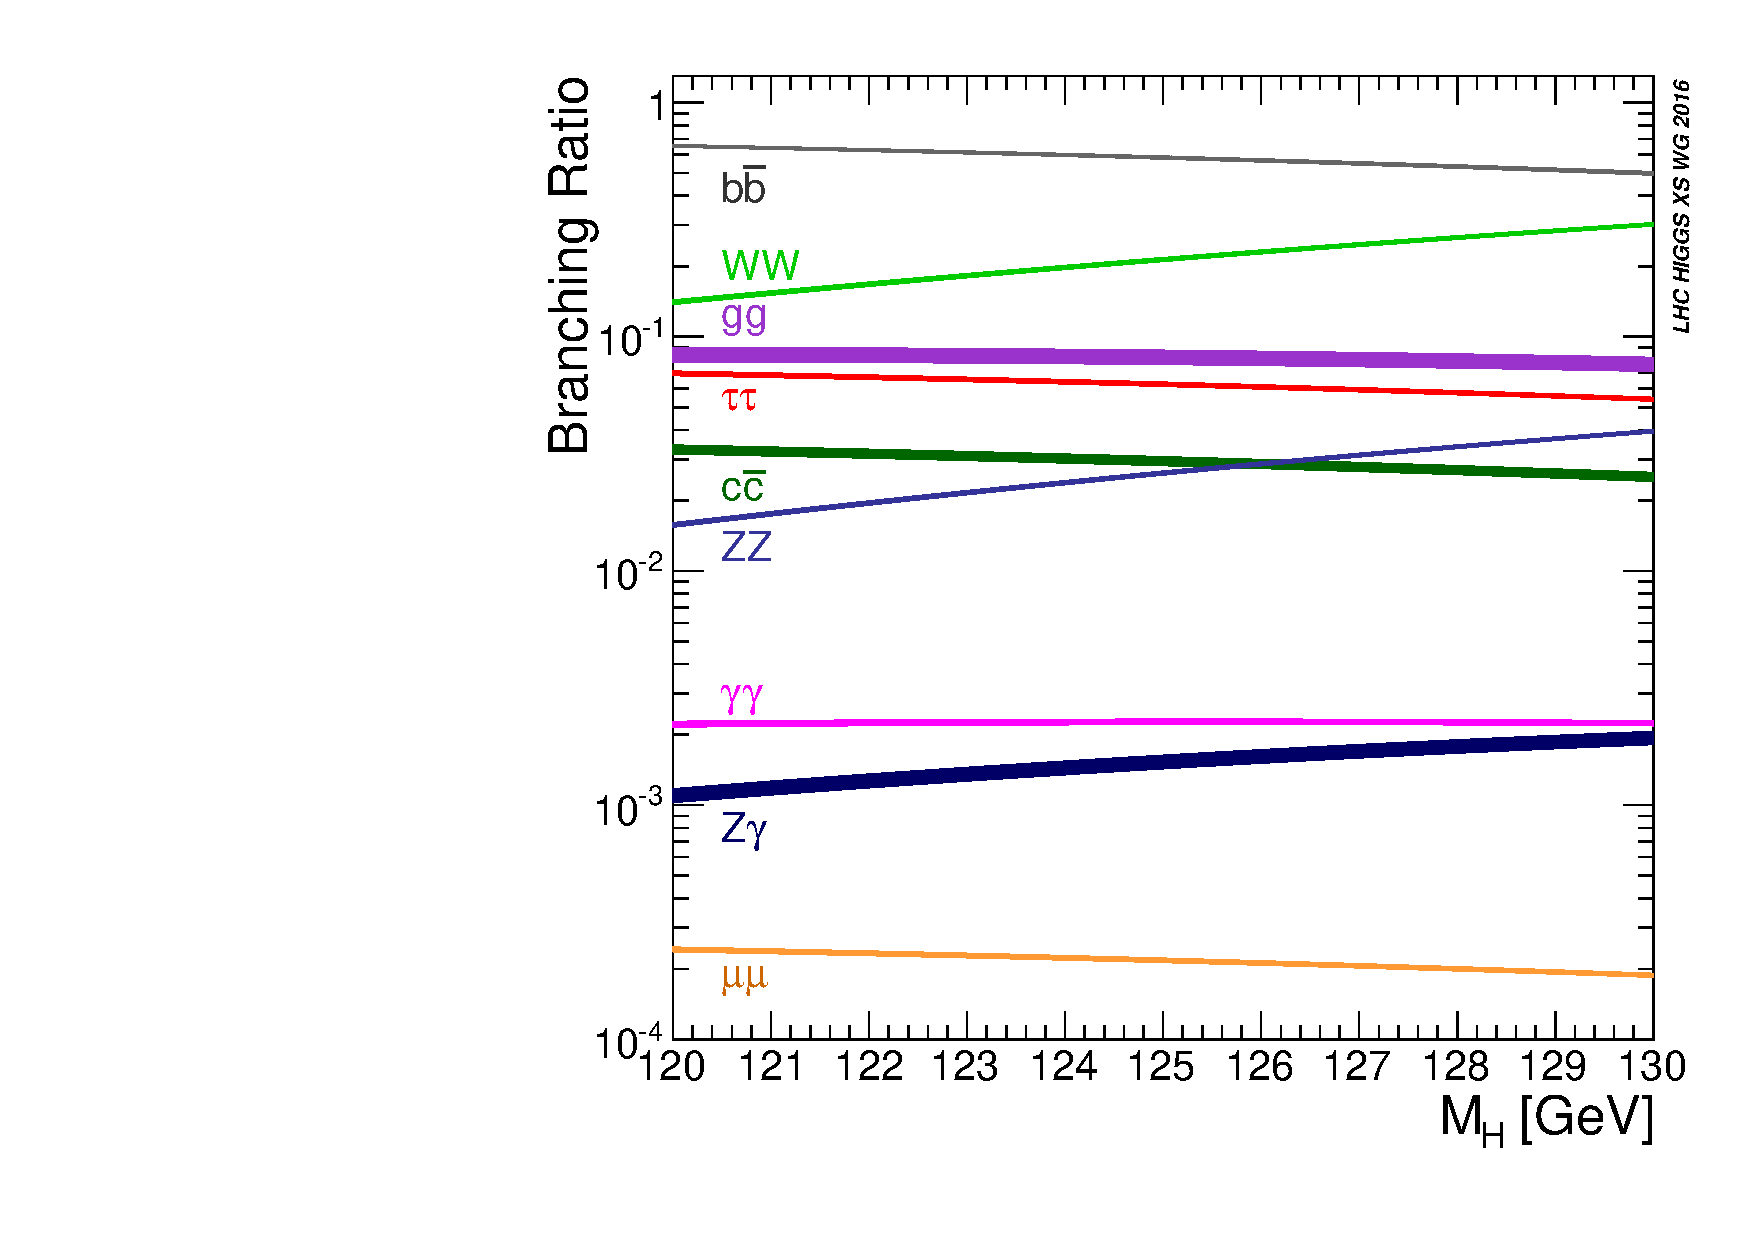
\includegraphics[width=0.65\textwidth]{phenomenology_of_processes/plots/SMHiggsBR_YR4-square.pdf}
     \caption{
The different theorized Higgs boson decay process are shown as a 
as a function of the Higgs boson mass.
The CMS and ATLAS experiments have determined $\mH = 125.09\GeV$~\cite{Aad:2015zhl}.
     }
     \label{fig:higgs_decay}
\end{figure*}

The leading Higgs boson decay processes each have certain advantages and disadvantages
for measuring the properties of the Higgs boson. The dominant Higgs boson decay 
process, $\PH\to\bbbar$, comprises well over half of all Higgs boson decays yet suffers
from very large background processes, making it difficult to distinguish Higgs bosons.
Additionally, the $m_{\bar{b}b}$ resolution is limited, making the expected Higgs boson
signal a broad distribution on top of a large background~\cite{PDG}.
The $\PH\to\PW\PW$ process has a large branching ratio, but this is reduced after requiring
$\PW^{\pm}\to\ell^{\pm} + \bar{\nu}$ where $\ell$ is a charged lepton. Additionally, the presence of neutrinos
in the final state decreases the Higgs boson mass resolution, $\approx 20\% \, \mH$~\cite{PDG}.
The $\PH\to\Pg\Pg$ is an extraordinarily difficult process to attempt to observe at a
hadron collider because the final state provides no helpful handles to disentangle it from
the dominant multijet backgrounds. This processes is mediated through a quark loop just
like the $ggH$ process.

The $\htt$ process is the largest direct Higgs boson to leptons decay process.
This provides a unique opportunity to probe the Higgs boson Yukawa couplings to the leptons.
Both the $\PH\to\bbbar$ and $\htt$ processes can directly probe the Higgs boson
Yukawa couplings to fermions. 
The mass resolution for the Higgs boson reconstructed from the $\htt$ process suffers like
the previously mentioned decays. The neutrinos resulting from the decay of the $\Pgt$
leptons make the mass reconstruction non-trivial.
The relative size of the backgrounds with event signatures similar to the Higgs boson
are much smaller than those for the $\PH\to\bbbar$ process. This is one
of the significant benefits of studying the Higgs boson through the $\htt$ process.

In this thesis, the various Higgs boson production cross sections and branching ratios
for Higgs boson production, and their corresponding uncertainties are taken from 
References~\cite{deFlorian:2016spz,Denner:2011mq,Ball:2011mu} and references therein.


\section{Higgs Boson: Experimental Results}
Searches for the Higgs boson were conducted at multiple experiments such as the searches
at the LEP at CERN in the 1990s~\cite{Barate:2000ts,Abdallah:2003ip,Achard:2001pj,Abbiendi:2000ac}.
In the datasets corresponding to these searches, there were not enough potential Higgs
boson events for discovery.
Instead, these searches all resulted in placing limits on the possible mass and cross section
of the Higgs boson. The Tevatron at Fermilab was active in Higgs boson searches through the early 2000s
with multiple analyses targeting the same decay process studied in this thesis, $\htt$. 
Similar to the LEP results, these analyses
placed limits on the possible mass and cross section of the Higgs boson~\cite{Aaltonen:2012jh, Abazov:2012zj}.
After the full analysis of the Tevatron dataset, there was evidence for the existance of a Higgs 
boson~\cite{PhysRevD.88.052014, PhysRevLett.109.071804}. However,
just like LEP, there were not enough potential Higgs boson events to qualify as a discovery.

The discovery of the Higgs boson required higher collision energies than those provided
by the Tevatron, which reached a maximum center-of-mass collision energy of 1.96\TeV. The
LHC at CERN was designed to deliver this increase in collision energy and in 2010 the LHC started
delivering proton-proton collisions at up to 7\TeV; an increase to 8\TeV followed in 2012.
Using the proton-proton collision data with center-of-mass energy 7 and 8\TeV,
a particle compatible with the Higgs boson expectations was observed by the CMS and ATLAS experiments at the CERN LHC
in events where the Higgs boson decays to $\PZ\PZ$, $\Pgg\Pgg$, and 
$\PW\PW$~\cite{Aad:2012tfa, Chatrchyan:2012xdj, Chatrchyan:2013lba}.

Using this same set of data, other analysts pursued the $\htt$ decay process and
the CMS Collaboration showed evidence for the $\htt$ process with an observed
significance of 3.2 based on an expected significance of 3.7 standard deviations (s.d.)
for a Higgs boson mass of 125\GeV~\cite{Chatrchyan:2014nva}.
The ATLAS experiment reported evidence for the $\htt$ process 
with an observed (expected) significance of 4.5\,(3.4)
s.d. for a Higgs boson mass of 125\GeV~\cite{Aad:2015vsa}.
The combination of results from both experiments yields an observed (expected)
significance of 5.5\,(5.0) s.d.~\cite{Khachatryan:2016vau}.

Further analysis from both experiments, described in References~\cite{Aad:2015gba, Khachatryan:2014jba, 
Chatrchyan:2012jja, Aad:2013xqa, Khachatryan:2014kca,Sirunyan:2017exp},
established that the measured properties of the new particle,
including its spin, charge-parity properties, and coupling strengths to SM particles, 
are consistent with those expected for the Higgs boson predicted by the SM.
The mass of the Higgs boson ($\mH$) has been determined to be
$125.09\pm0.21\stat\pm0.11\syst\GeV$, from a combination of
ATLAS and CMS measurements~\cite{Aad:2015zhl}. An example of these measurements
can be seen in Figure~\ref{fig:run_1_comb_mu} which shows the best fit value for the signal
strength for the Higgs boson production and decay processes. As can be seen, the
majority of the $\Pgt\Pgt$ decay process measurements shows agreement with the SM predictions for the Higgs
boson. The measurements corresponding to $\htt$ with the Higgs bosons produced in association
with a $\PW$ boson ($\PW\PH$) and the measurement of the Higgs boson produced with
two top-quarks ($\ttbar\PH$) show non-significant deviation from the SM prediction. However, 
the uncertainties are sizable and are represented by the size of the 1$\sigma$ band. 
These $\ttbar\PH$ Run-I results have been updated with the same dataset studied in this thesis.
The updated $\ttbar\PH$, $\htt$ results are compatible with the SM prediction within 1$\sigma$~\cite{Sirunyan:2018hoz}.
Further data collection and analysis
will continue to reduce the size of the 1$\sigma$ uncertainty bands and will show if 
deviations are statistically significant or if they are 
temporary fluctuations that are smoothed out with more data collection.

\begin{figure*}[htbp]
\centering
     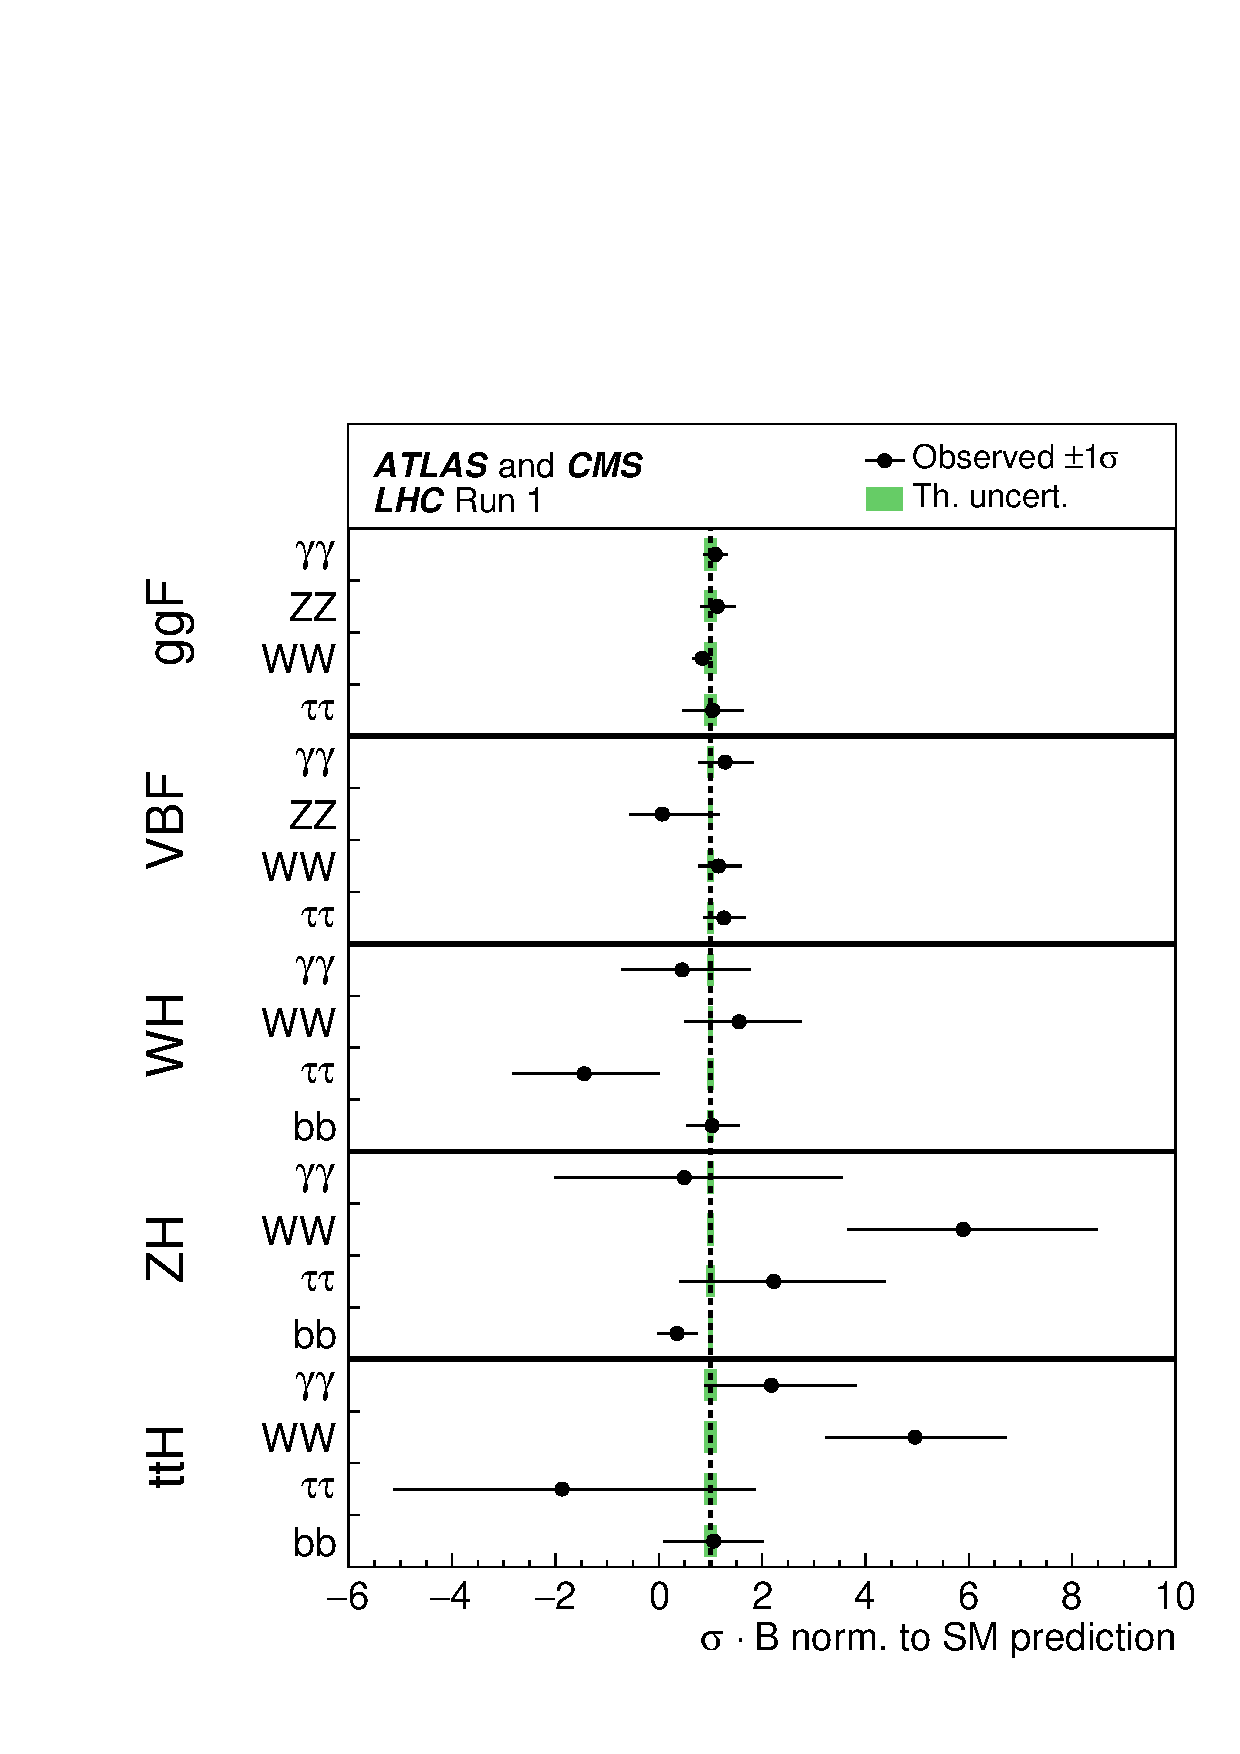
\includegraphics[width=0.6\textwidth]{introduction/plots/run_1_comb_mu.pdf}
     \caption{
The best fit values for the signal strength of the listed Higgs boson production
processes and decay processes. A value of 1 indicates perfect agreement with the SM.
The error bars indicate the 1$\sigma$ intervals. The green shaded bands indicate the
theoretical uncertainties in the predictions.
     }
     \label{fig:run_1_comb_mu}
\end{figure*}

This thesis builds on these previous experimental results at 7 and 8\TeV and measures the
properties of the Higgs boson in the $\htt$ decay process at 13\TeV center-of-mass 
collision energy. We establish the first 13\TeV observation of the $\htt$
process with an observed (expected) significance of 5.5\,(4.8) s.d.~\cite{HIG-18-007}. 
The best fit signal strengths are measured similar
to what is seen in Figure~\ref{fig:run_1_comb_mu}. Additionally, the couplings of the
Higgs boson to fermions and vector bosons is measured and is discussed in the final results
section of this thesis, Chapter~\ref{sec:cmb_results}.



